\documentclass{article}
\usepackage[utf8]{inputenc}
\usepackage[greek,english]{babel}
\usepackage{alphabeta}
\usepackage{fancyhdr}
\usepackage{listings}
\usepackage{mathtools}
\usepackage{xcolor}
\usepackage[backend=bibtex]{biblatex}
\usepackage{hyperref}
\usepackage[left=1cm,right=1cm]{geometry}
\hypersetup{
	colorlinks=true,
	linktoc=all,
	linkcolor=black,
}
\lstset {
        basicstyle=\ttfamily,
        columns=fullflexible,
        breaklines=true,
        keepspaces=true,
	showstringspaces=false
}

\title{Μικροϋπολογιστές: Εργαστηριακή άσκηση 7}
\author{Χρήστος Μαργιώλης -- 19390133}
\date{Ιανουάριος 2023}

\begin{document}

\begin{titlepage}
        \maketitle
\end{titlepage}

\section{Κύκλωμα}

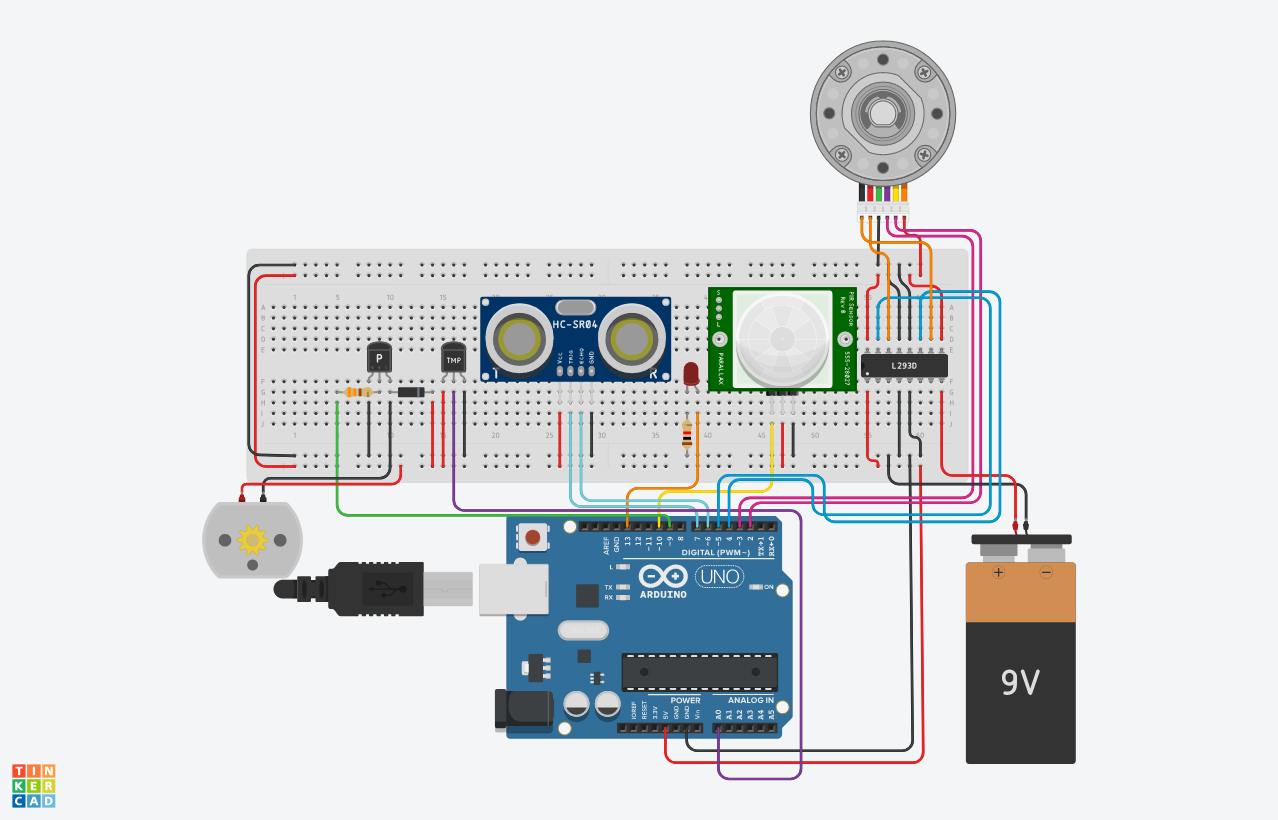
\includegraphics[width=\linewidth]{door.png}
\pagebreak

\section{Κώδικας}

\lstinputlisting[language=C]{door.ino}

\end{document}
